\chapter{Testing and Continuous Integration}
\label{chapter:testingAndCI}

Implemented functionality should always be tested. Not only to ensure that it does what it is supposed to do, but also to avoid regression. Nothing is worse than introducing a bug by implementing a new feature without noticing it. Therefore, unit, snapshot and end-to-end tests are used to avoid regression in this project.
Moreover, all tests are run on each commit to the GitLab repository.

\section{Testing}
\label{section:testing}
For unit and snapshot testing Jest is used. Jest is a JavaScript testing framework focusing on simplicity and is maintained by Facebook. It requires zero configuration, runs tests in isolation and can therefore be parallelized \cite{Jest}. For end-to-end testing Nightwatch is used. Nightwatch is a Node.js powered end-to-end testing framework for web applications. It supports testing in Chrome, Firefox and Edge, has the concept of page objects to easily abstract the content of a page and allows extending the framework with custom commands \cite{Nightwatch}.

\subsection{Unit Testing}
\label{subsection:unitTesting}
Unit tests are used to verify the correctness of individual functions and apply the following concept: the tester has an input to a function and knows what the function should output for this input. The tester then compares the actual output of the function and compares it to the expected output. If those are not the same the test is evaluated as failed, and succeeds otherwise.

There are two main categories of unit tests: black-box and white-box testing.

\subsection*{Black-box and White-box Testing}
Black-box testing is a testing method where the tester does not know how a function is implemented, but knows its specification and creates tests based on this knowledge. White-box testing on the other hand is a testing method where the tester does know the implementation of the function. Usually, both kinds of software testing should be used, but since there are no software testers (testers applying black-box testing) involved in this project, only white-box testing is applied \cite{BlackBoxWhiteBoxTesting}.

\subsection*{Test Plan}

General purpose components are tested on their respective functionality, i.e whether they react correctly to different user inputs. The tests for a component representing an exercise check whether:

\begin{itemize}
    \item Initial conditions hold
    \item Various exercise-specific user inputs are handled correctly
    \item Restarting the exercise works as expected
    \item Starting the next example cleans up everything from previous exercise
    \item The correct answer is accepted
    \item Incorrect answers are rejected
\end{itemize}

\subsection*{Code Coverage}
As mentioned before, unit tests usually test at the function level. To catch as many possible code paths and edge cases, the same function is tested multiple times with different inputs. 
A metric to judge the usefulness of a test suite is code coverage. Usually, a coverage report includes:

\begin{itemize}
    \item \textbf{Statement coverage} - The percentage of statements that have been executed 
    \item \textbf{Branch coverage} - The percentage of branches of the control structures (e.g. if and loop statements) that have been executed
    \item \textbf{Function coverage} - The percentage of functions that have been called
    \item \textbf{Lines coverage} - The percentage of lines of the source code that have been executed
\end{itemize}

High coverage percentage does not imply that it is a good test suite. Some critical paths can still be untested. It is generally accepted that a code coverage of 80\% is a desirable goal. Going above 80\% of code coverage is usually costly and doesn't provide much additional benefit \cite{CodeCoverage}.

The code coverage for the whole project and each component is given in table \ref{table:testCoverage}. Most of the components are well tested with a code coverage of above 80\% in most categories. Some rows in table \ref{table:testCoverage} indicate bad code coverage. Usually those components with bad code coverage have fewer than forty lines and are therefore not tested thoroughly. 
 
\subsection*{Non-determinism}
A problem that has to be tackled for testing is how to handle non-determinism. Some exercises are based on random behaviour to achieve a rich user experience. However, if random behaviour is used, the actual output may not be the same as the expected output and the test is incorrectly evaluated as failed. To avoid this issue, one can mock the function that is used to generate random numbers. Mock functions allow to overwrite the actual implementation of the function by intercepting calls to this function and return values configured by the test suite \cite{Jest}. For this reason, there is a function to generate random numbers in \nameref{subsection:gameMixin}.

\begin{table}
    \begin{adjustwidth}{-2cm}{}
        \caption{Test coverage of all components}
        \centering
        \begin{tabular}{|l|l|l|l|l|}
        \hline
            File & \% Statements & \% Branches & \% Functions & \% Lines \\ \hline
            All files & 86.71 & 73.11 & 86.73 & 86.56 \\ \hline
            App.vue & 100 & 100 & 100 & 100 \\ \hline
            GameMixins.vue & 55.56 & 100 & 27.27 & 55.56 \\ \hline
            Home.vue & 100 & 100 & 100 & 100 \\ \hline
            ciphertexts/PatternEncryption.vue & 79.41 & 50 & 81.82 & 78.13 \\ \hline
            ciphertexts/PatternDecryption.vue & 78.79 & 50 & 80 & 77.42 \\ \hline
            layout/Footer.vue & 100 & 100 & 100 & 100 \\ \hline
            layout/Header.vue & 100 & 100 & 100 & 100 \\ \hline
            numbersystems/From.vue & 100 & 100 & 100 & 100 \\ \hline
            numbersystems/ItemDropzone.vue & 100 & 100 & 100 & 100 \\ \hline
            numbersystems/ItemGroup.vue & 100 & 100 & 100 & 100 \\ \hline
            numbersystems/NumbersystemsMixin.vue & 75.41 & 62.5 & 84.62 & 77.59 \\ \hline
            numbersystems/Swap.vue & 88.89 & 83.33 & 88.89 & 91.18 \\ \hline
            numbersystems/To.vue & 90.24 & 45.45 & 90 & 92.11 \\ \hline
            shared/Buttonmenu.vue & 66.67 & 100 & 0 & 66.67 \\ \hline
            shared/Difficulty.vue & 87.5 & 62.5 & 100 & 87.5 \\ \hline
            shared/ItemSelection.vue & 100 & 100 & 100 & 100 \\ \hline
            shared/Modal.vue & 100 & 100 & 100 & 100 \\ \hline
            shared/Trashcan.vue & 100 & 100 & 100 & 100 \\ \hline
            shared/Tutorial.vue & 100 & 100 & 100 & 100 \\ \hline
            shared/Undo.vue & 100 & 100 & 100 & 100 \\ \hline
            trees/Row.vue & 89.04 & 65.71 & 100 & 88.89 \\ \hline
            trees/Sudoku.vue & 91.12 & 76.09 & 94.12 & 90.26 \\ \hline
            trees/TreesMixin.vue & 100 & 100 & 100 & 100 \\ \hline
            words/Add.vue & 98.33 & 100 & 95.24 & 98.28 \\ \hline
            words/Change.vue & 91.43 & 83.33 & 93.33 & 91.18 \\ \hline
            words/Remove.vue & 100 & 100 & 100 & 100 \\ \hline
            words/Swap.vue & 61.22 & 87.5 & 76 & 59.78 \\ \hline
        \end{tabular}
        \label{table:testCoverage}
    \end{adjustwidth}
\end{table}

\subsection{Snapshot Testing}
\label{subsection:snapshotTesting}
Snapshot tests ensure correctness of the user interface and show an alert when it changes unexpectedly. More precisely, snapshot tests render the template of a component to HTML, take a snapshot and compare the snapshot with the previously saved reference snapshot. These two snapshots are compared. If they don't match, the test fails. Otherwise the test succeeds. If the changes made to the source code were intended to change the UI, the snapshot has to be updated. This requires an initial snapshot that is known to be correct. Hence, snapshots should be committed to the repository as well \cite{Jest}.

Every component in this project is snapshot tested and is therefore safe from unintended UI changes.

\subsection{End-to-End Testing}
\label{subsection:e2e}
End-to-end tests are used to test the entire application flow. The main goal is to test it from a user's perspective by simulating the interactions of a use case \cite{EndToEndTests}. 

Nightwatch allows to run end-to-end tests for Chrome, Firefox and Edge to ensure the application works across browser-borders. The end-to-end tests for this project make use of page objects. A page object is an abstraction of a page represented as an object. Its goal is to simplify the end-to-end test \cite{Nightwatch}.

Many exercises are based on non-determinism, which a user cannot influence. Thus, the end-to-end tests aren't able to, either. Therefore, the end-to-end tests in this project cover all parts of an exercise one needs to see to solve it. 

\section{Continuous Integration}
\label{section:CI}

This project make use of the GitLab Continuous Integration (CI). When pushing a commit to the project's GitLab repository, the CI pipeline is run (figure \ref{fig:pipeline}). The CI pipeline is specified in the \code{.gitlab-ci.yml} file in the project's root folder, which specifies which jobs need to be executed. Usually, these jobs build, test and validate changes made to the source code and allow to easily catch bugs and errors.
The CI pipeline of this project consists of two parts:

\begin{itemize}
    \item \textbf{Unit and Snapshot tests} - runs the unit and snapshot tests as described in \nameref{subsection:unitTesting} and \nameref{subsection:snapshotTesting}
    \item \textbf{End-to-end tests} - runs the end-to-end tests as described in \nameref{subsection:e2e}
\end{itemize}

\begin{figure} 
    \centering
    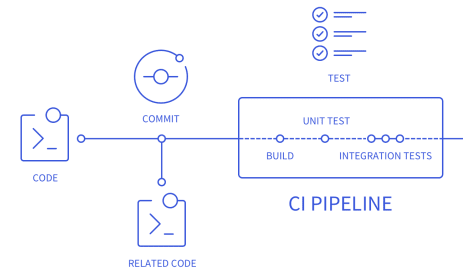
\includegraphics[width=0.6 \columnwidth]{figures/pipeline.png}
    \caption{Pipeline visualization \cite{CIPipeline}} 
    \label{fig:pipeline} 
\end{figure}